\documentclass{standalone}
\usepackage{tikz}
\usetikzlibrary{patterns, positioning}
\usepackage[sfdefault]{ClearSans} %% option 'sfdefault' activates Clear Sans as the default text font
\usepackage[T1]{fontenc}

\begin{document}
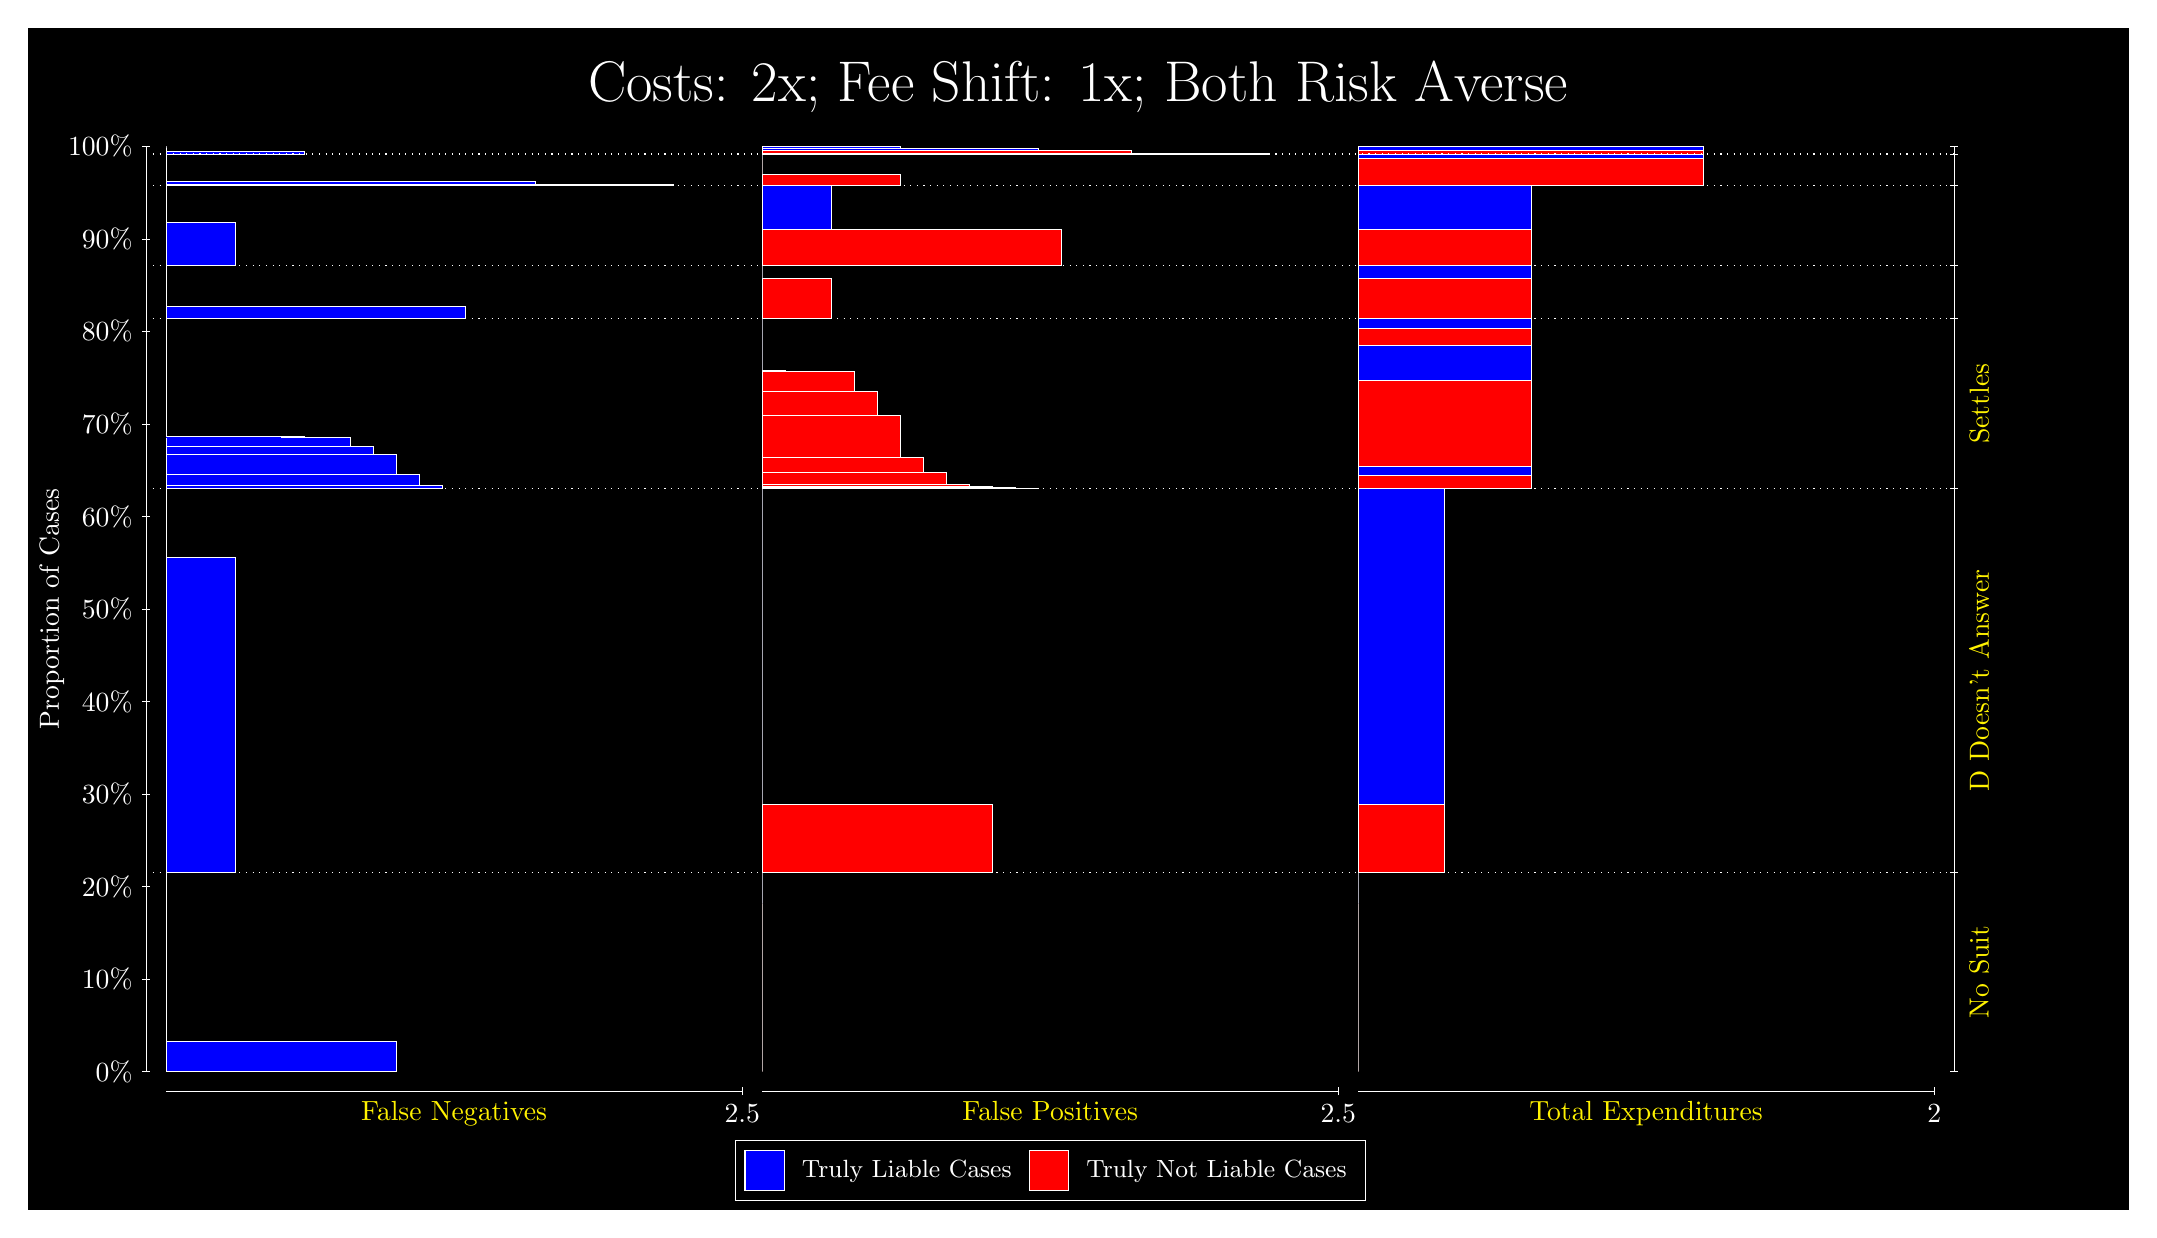
\begin{tikzpicture}
\draw[fill=black] (0,0) rectangle (26.667,15);
\draw[text=white] (0,13.5) rectangle (26.667,15) node[midway] {\huge Costs: 2x; Fee Shift: 1x; Both Risk Averse};
\draw[white, very thin] (1.5,1.75) -- (1.5,13.5);
\node[rotate=90, text=white, anchor=center] at (0.3, 7.625) {Proportion of Cases};
\draw[white, very thin] (1.45,1.75) -- (1.55,1.75);
\node[text=white, anchor=east] at (1.45, 1.75) {0\%};
\draw[white, very thin] (1.45,2.925) -- (1.55,2.925);
\node[text=white, anchor=east] at (1.45, 2.925) {10\%};
\draw[white, very thin] (1.45,4.1) -- (1.55,4.1);
\node[text=white, anchor=east] at (1.45, 4.1) {20\%};
\draw[white, very thin] (1.45,5.275) -- (1.55,5.275);
\node[text=white, anchor=east] at (1.45, 5.275) {30\%};
\draw[white, very thin] (1.45,6.45) -- (1.55,6.45);
\node[text=white, anchor=east] at (1.45, 6.45) {40\%};
\draw[white, very thin] (1.45,7.625) -- (1.55,7.625);
\node[text=white, anchor=east] at (1.45, 7.625) {50\%};
\draw[white, very thin] (1.45,8.8) -- (1.55,8.8);
\node[text=white, anchor=east] at (1.45, 8.8) {60\%};
\draw[white, very thin] (1.45,9.975) -- (1.55,9.975);
\node[text=white, anchor=east] at (1.45, 9.975) {70\%};
\draw[white, very thin] (1.45,11.15) -- (1.55,11.15);
\node[text=white, anchor=east] at (1.45, 11.15) {80\%};
\draw[white, very thin] (1.45,12.325) -- (1.55,12.325);
\node[text=white, anchor=east] at (1.45, 12.325) {90\%};
\draw[white, very thin] (1.45,13.5) -- (1.55,13.5);
\node[text=white, anchor=east] at (1.45, 13.5) {100\%};

\draw[white, very thin] (24.457,1.75) -- (24.457,13.5);
\draw[white, very thin] (24.407,1.75) -- (24.507,1.75);
\node[anchor=west] at (24.407, 1.75) {};
\draw[white, very thin] (24.407,4.2758) -- (24.507,4.2758);
\node[anchor=west] at (24.407, 4.2758) {};
\draw[white, very thin] (24.407,9.1518) -- (24.507,9.1518);
\node[anchor=west] at (24.407, 9.1518) {};
\draw[white, very thin] (24.407,11.31) -- (24.507,11.31);
\node[anchor=west] at (24.407, 11.31) {};
\draw[white, very thin] (24.407,11.984) -- (24.507,11.984);
\node[anchor=west] at (24.407, 11.984) {};
\draw[white, very thin] (24.407,13.004) -- (24.507,13.004);
\node[anchor=west] at (24.407, 13.004) {};
\draw[white, very thin] (24.407,13.402) -- (24.507,13.402);
\node[anchor=west] at (24.407, 13.402) {};
\draw[white, very thin] (24.407,13.5) -- (24.507,13.5);
\node[anchor=west] at (24.407, 13.5) {};

\draw[white, very thin, fill=blue] (1.75,1.75) rectangle (4.6775,2.1391);
\draw[white, very thin, fill=red] (1.75,2.1391) rectangle (1.75,4.2758);
\draw[white, very thin, fill=blue] (1.75,4.2758) rectangle (2.6283,8.2779);
\draw[white, very thin, fill=red] (1.75,8.2779) rectangle (1.75,9.1518);
\draw[white, very thin, fill=blue] (1.75,9.1518) rectangle (5.2631,9.1963);
\draw[white, very thin, fill=blue] (1.75,9.1963) rectangle (4.9703,9.3317);
\draw[white, very thin, fill=blue] (1.75,9.3317) rectangle (4.6775,9.587);
\draw[white, very thin, fill=blue] (1.75,9.587) rectangle (4.3848,9.5906);
\draw[white, very thin, fill=blue] (1.75,9.5906) rectangle (4.3848,9.6967);
\draw[white, very thin, fill=blue] (1.75,9.6967) rectangle (4.092,9.7986);
\draw[white, very thin, fill=blue] (1.75,9.7986) rectangle (3.7993,9.8063);
\draw[white, very thin, fill=blue] (1.75,9.8063) rectangle (3.5065,9.8119);
\draw[white, very thin, fill=blue] (1.75,9.8119) rectangle (3.2138,9.814);
\draw[white, very thin, fill=blue] (1.75,9.814) rectangle (2.921,9.8174);
\draw[white, very thin, fill=red] (1.75,9.8174) rectangle (1.75,11.31);
\draw[white, very thin, fill=blue] (1.75,11.31) rectangle (5.5558,11.472);
\draw[white, very thin, fill=red] (1.75,11.472) rectangle (1.75,11.984);
\draw[white, very thin, fill=blue] (1.75,11.984) rectangle (2.6283,12.54);
\draw[white, very thin, fill=red] (1.75,12.54) rectangle (1.75,13.004);
\draw[white, very thin, fill=blue] (1.75,13.004) rectangle (8.1906,13.024);
\draw[white, very thin, fill=blue] (1.75,13.024) rectangle (6.4341,13.058);
\draw[white, very thin, fill=red] (1.75,13.058) rectangle (1.75,13.402);
\draw[white, very thin, fill=blue] (1.75,13.402) rectangle (3.5065,13.433);
\draw[white, very thin, fill=red] (1.75,13.433) rectangle (1.75,13.485);
\draw[white, very thin, fill=blue] (1.75,13.485) rectangle (1.75,13.5);
\draw[white, very thin, fill=red] (9.3189,1.75) rectangle (9.3189,3.8867);
\draw[white, very thin, fill=blue] (9.3189,3.8867) rectangle (9.3189,4.2758);
\draw[white, very thin, fill=red] (9.3189,4.2758) rectangle (12.246,5.1497);
\draw[white, very thin, fill=blue] (9.3189,5.1497) rectangle (9.3189,9.1518);
\draw[white, very thin, fill=red] (9.3189,9.1518) rectangle (12.832,9.1586);
\draw[white, very thin, fill=red] (9.3189,9.1586) rectangle (12.539,9.1647);
\draw[white, very thin, fill=red] (9.3189,9.1647) rectangle (12.246,9.1803);
\draw[white, very thin, fill=red] (9.3189,9.1803) rectangle (11.954,9.206);
\draw[white, very thin, fill=red] (9.3189,9.206) rectangle (11.661,9.3562);
\draw[white, very thin, fill=red] (9.3189,9.3562) rectangle (11.368,9.5566);
\draw[white, very thin, fill=red] (9.3189,9.5566) rectangle (11.075,10.081);
\draw[white, very thin, fill=red] (9.3189,10.081) rectangle (10.783,10.395);
\draw[white, very thin, fill=red] (9.3189,10.395) rectangle (10.49,10.644);
\draw[white, very thin, fill=blue] (9.3189,10.644) rectangle (9.9044,10.647);
\draw[white, very thin, fill=blue] (9.3189,10.647) rectangle (9.6116,10.65);
\draw[white, very thin, fill=blue] (9.3189,10.65) rectangle (9.3189,11.31);
\draw[white, very thin, fill=red] (9.3189,11.31) rectangle (10.197,11.821);
\draw[white, very thin, fill=blue] (9.3189,11.821) rectangle (9.3189,11.984);
\draw[white, very thin, fill=red] (9.3189,11.984) rectangle (13.125,12.448);
\draw[white, very thin, fill=blue] (9.3189,12.448) rectangle (10.197,13.004);
\draw[white, very thin, fill=red] (9.3189,13.004) rectangle (11.075,13.148);
\draw[white, very thin, fill=red] (9.3189,13.148) rectangle (9.3189,13.349);
\draw[white, very thin, fill=blue] (9.3189,13.349) rectangle (9.3189,13.402);
\draw[white, very thin, fill=red] (9.3189,13.402) rectangle (15.759,13.41);
\draw[white, very thin, fill=red] (9.3189,13.41) rectangle (14.003,13.454);
\draw[white, very thin, fill=blue] (9.3189,13.454) rectangle (12.832,13.469);
\draw[white, very thin, fill=blue] (9.3189,13.469) rectangle (11.075,13.5);
\draw[white, very thin, fill=red] (16.888,1.75) rectangle (16.888,3.8867);
\draw[white, very thin, fill=blue] (16.888,3.8867) rectangle (16.888,4.2758);
\draw[white, very thin, fill=red] (16.888,4.2758) rectangle (17.986,5.1497);
\draw[white, very thin, fill=blue] (16.888,5.1497) rectangle (17.986,9.1518);
\draw[white, very thin, fill=red] (16.888,9.1518) rectangle (19.083,9.3237);
\draw[white, very thin, fill=blue] (16.888,9.3237) rectangle (19.083,9.4333);
\draw[white, very thin, fill=red] (16.888,9.4333) rectangle (19.083,10.535);
\draw[white, very thin, fill=blue] (16.888,10.535) rectangle (19.083,10.974);
\draw[white, very thin, fill=red] (16.888,10.974) rectangle (19.083,11.192);
\draw[white, very thin, fill=blue] (16.888,11.192) rectangle (19.083,11.31);
\draw[white, very thin, fill=red] (16.888,11.31) rectangle (19.083,11.821);
\draw[white, very thin, fill=blue] (16.888,11.821) rectangle (19.083,11.984);
\draw[white, very thin, fill=red] (16.888,11.984) rectangle (19.083,12.448);
\draw[white, very thin, fill=blue] (16.888,12.448) rectangle (19.083,13.004);
\draw[white, very thin, fill=red] (16.888,13.004) rectangle (21.279,13.349);
\draw[white, very thin, fill=blue] (16.888,13.349) rectangle (21.279,13.402);
\draw[white, very thin, fill=red] (16.888,13.402) rectangle (21.279,13.454);
\draw[white, very thin, fill=blue] (16.888,13.454) rectangle (21.279,13.5);
\draw[white, dotted] (1.5,4.2758) -- (24.457,4.2758);
\draw[white, dotted] (1.5,9.1518) -- (24.457,9.1518);
\draw[white, dotted] (1.5,11.31) -- (24.457,11.31);
\draw[white, dotted] (1.5,11.984) -- (24.457,11.984);
\draw[white, dotted] (1.5,13.004) -- (24.457,13.004);
\draw[white, dotted] (1.5,13.402) -- (24.457,13.402);
\draw[white, very thin] (1.75,1.5) -- (9.0689,1.5);
\node[text=yellow, anchor=north] at (5.4094, 1.5) {False Negatives};
\draw[white, very thin] (9.0689,1.45) -- (9.0689,1.55);
\node[text=white, anchor=north] at (9.0689, 1.45) {2.5};

\draw[white, very thin] (9.3189,1.5) -- (16.638,1.5);
\node[text=yellow, anchor=north] at (12.978, 1.5) {False Positives};
\draw[white, very thin] (16.638,1.45) -- (16.638,1.55);
\node[text=white, anchor=north] at (16.638, 1.45) {2.5};

\draw[white, very thin] (16.888,1.5) -- (24.207,1.5);
\node[text=yellow, anchor=north] at (20.547, 1.5) {Total Expenditures};
\draw[white, very thin] (24.207,1.45) -- (24.207,1.55);
\node[text=white, anchor=north] at (24.207, 1.45) {2};

\node[text=yellow, centered, rotate=90] at (24.777, 3.0129) {No Suit};
\node[text=yellow, centered, rotate=90] at (24.777, 6.7138) {D Doesn't Answer};
\node[text=yellow, centered, rotate=90] at (24.777, 10.231) {Settles};





\draw (12.978300999999998,1.5) node[draw=none] (baseCoordinate) {};
\begin{scope}[align=center]
        \matrix[scale=0.5, draw=white, below=0.5cm of baseCoordinate, nodes={draw}, column sep=0.1cm]{
            \node[rectangle, draw, minimum width=0.5cm, minimum height=0.5cm, fill=blue] {}; &
            \node[draw=none, font=\small, text=white] (B) {Truly Liable Cases}; &
            \node[rectangle, draw, minimum width=0.5cm, minimum height=0.5cm, fill=red] {}; &
            \node[draw=none, font=\small, text=white] (B) {Truly Not Liable Cases}; \\
            };
\end{scope}

\end{tikzpicture}
\end{document}